% Table generated by Excel2LaTeX from sheet 'Sheet1'
%
\begin{table}
   \tiny
   \centering
   \noindent
    \caption[Phage elements in {\it S.} Typhimurium]{\textbf{Phage elements in {\it S.} Typhimurium.} Genomic coordinates determined from annotations in the EMBL annotation for FQ312003 and manual inspection. Repressor domains and architecture were determined using the HMMER webserver \parencite{Finn2011} and Pfam \parencite{Punta2012}. Phage types were determined using repressor sequence similarity searches and information from \textcite{Thomson2004} and \textcite{Kropinski2007}. }
    \begin{tabular}{     m{0.5in}
    				m{0.4in}
				m{0.4in}
				m{0.6in}
				m{1.6in}
				m{0.4in}
				m{0.5in}
				m{0.5in}
				}
   
    \\
     \toprule
    \textbf{Element name} & \textbf{Genomic coordinates} & \textbf{Repressor} & \textbf{Repressor domain(s)} & \textbf{Repressor domain architecture} & \textbf{Predicted active?} & \textbf{Phage type} & \textbf{Required cargo} \\
    \midrule
    Gifsy-2 SLP105 & 1054795 - 1100036 & SL0950 & HTH\_3 (PF01381) &
\includegraphics[height=6mm]{rep1}& Yes   & lambdoid & N/A \\
    N/A   & 1913364 - 1925490 & N/A   & N/A   & N/A   & No    & remnant & SL1799 \\
    SLP203 & 2039803 - 2079890 & SL1967 & HTH\_19 (PF12844) and Peptidase\_S24 (PF00717) &
\includegraphics[height=6mm]{rep2}& Yes   & P22-like & N/A \\
    Gifsy-1 SLP272 & 2726717 - 2777229 & SL2593 & HTH\_3 (PF01381) &    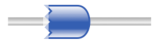
\includegraphics[height=6mm]{rep3}   & Yes   & lambdoid & SL2549 \\
    SLP281 & 2815382 - 2825915 & SL2633 & 2 X Phage\_CI\_repr (PF07022) &   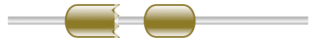
\includegraphics[height=6mm]{rep4}    & Yes   & degenerate P2-like & N/A \\
    Fels-2 SLP285 & 2855616 - 2888522 & SL2708 & Phage\_CI\_repr (PF07022) &   
\includegraphics[height=6mm]{rep5}    & Yes   & P2-like & SL2695 \\
    SLP289 & 2890073 - 2900377 & IsrK RNA (RF01394) & N/A   & N/A   & No    & P4-like & N/A \\
    SLP443 & 4437731 - 4459844 & N/A   & N/A   & N/A   & No    & remnant & SL4132 \\
    \bottomrule    
    \end{tabular}%
    \label{tab:stm_phage}%
\end{table}

